% Editable native annotations around unchanged verified IDE photographs.
\par
\begin{figure}[htbp]
\centering
\sbox0{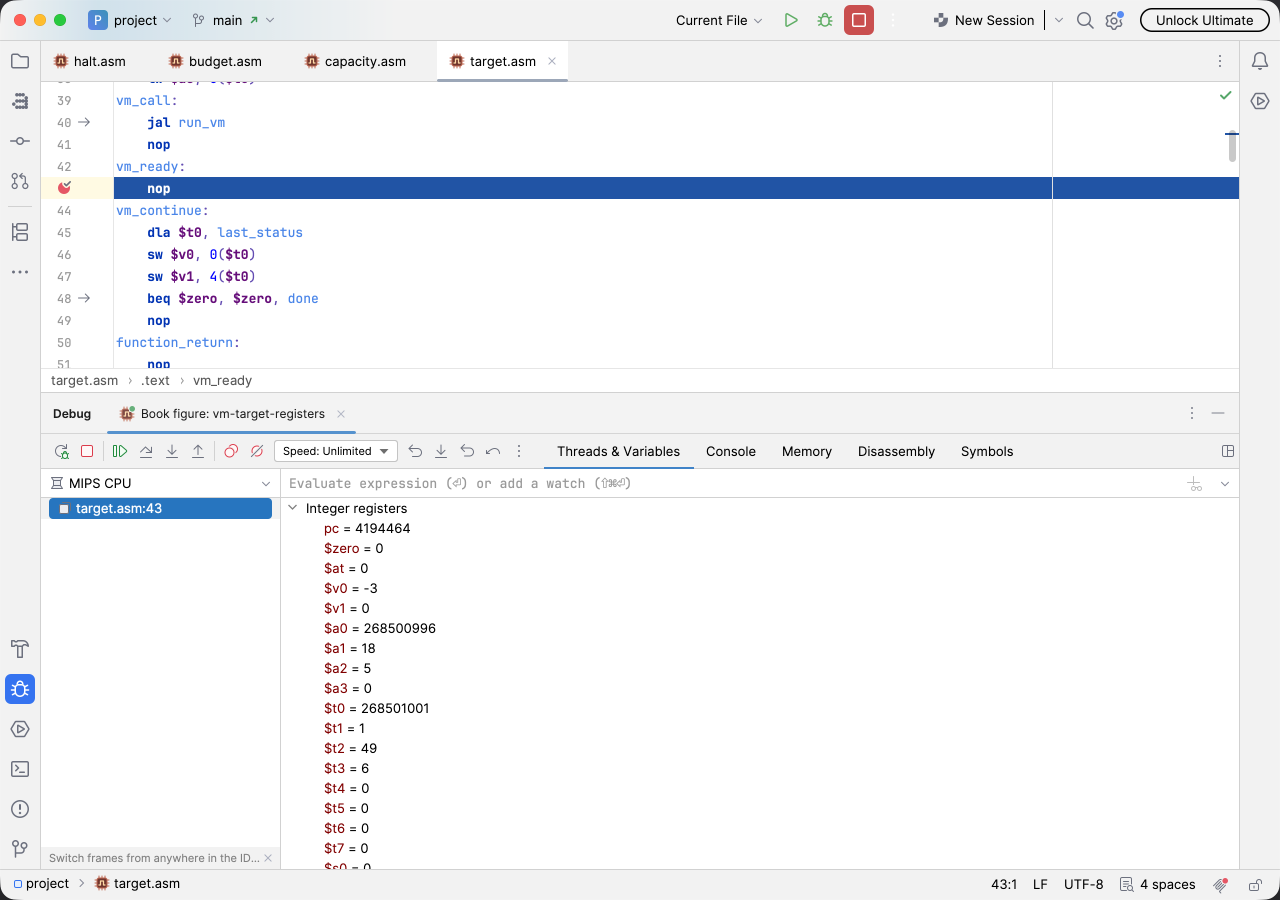
\includegraphics[artifact]{packages/018-tiny-bytecode-interpreter/captures/f04/registers.png}}
\sbox2{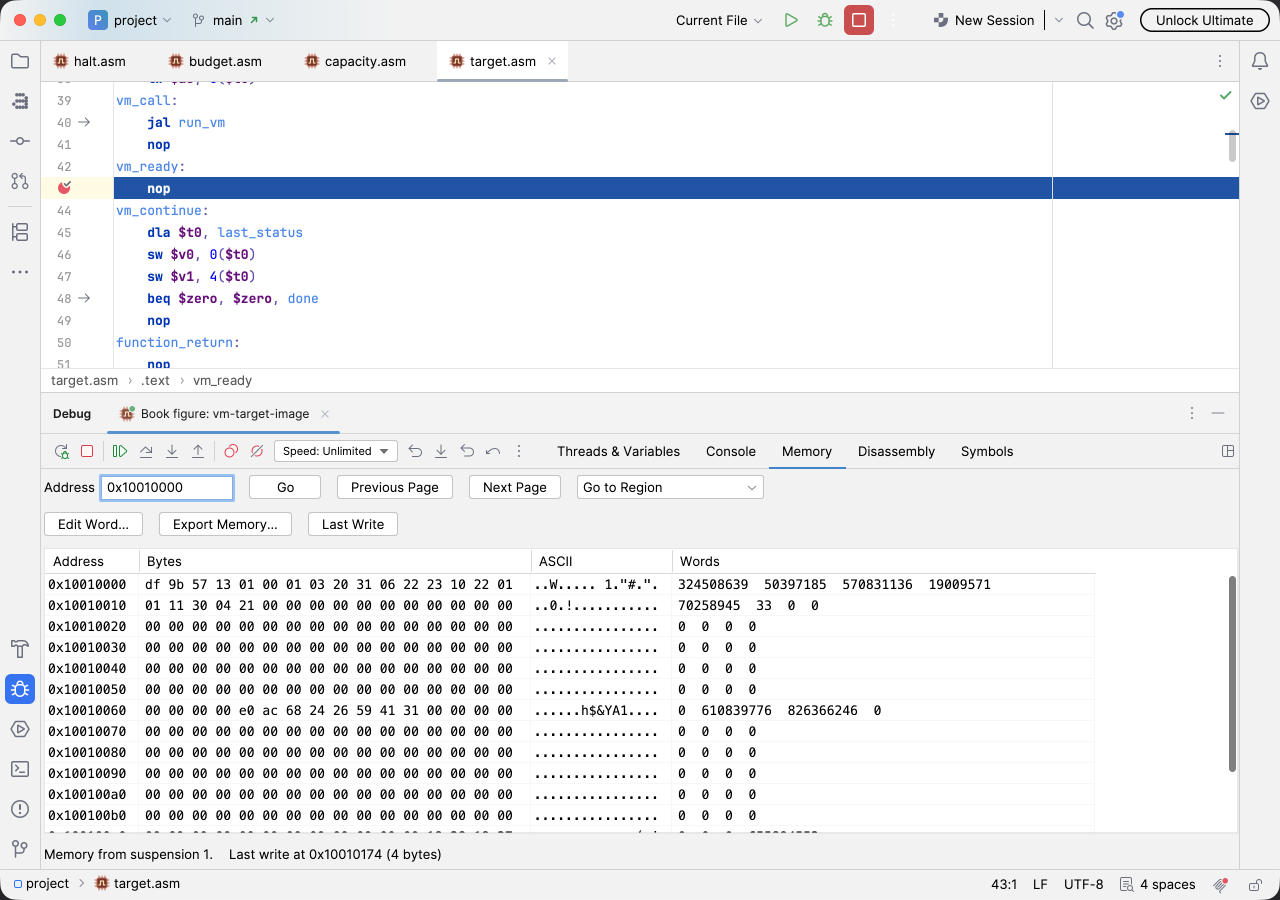
\includegraphics[artifact]{packages/018-tiny-bytecode-interpreter/captures/f04/image.png}}
\sbox4{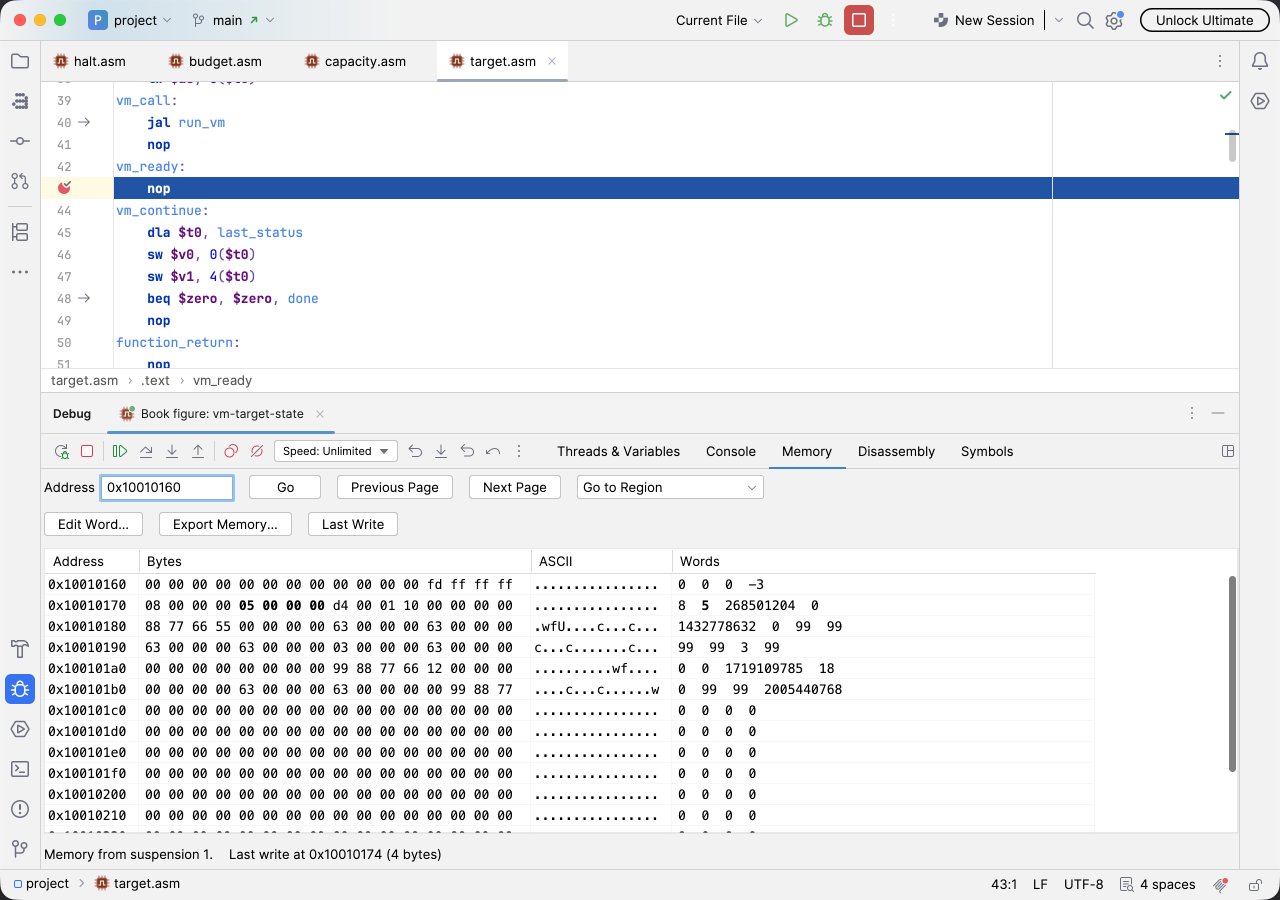
\includegraphics[artifact]{packages/018-tiny-bytecode-interpreter/captures/f04/state.png}}
\sbox6{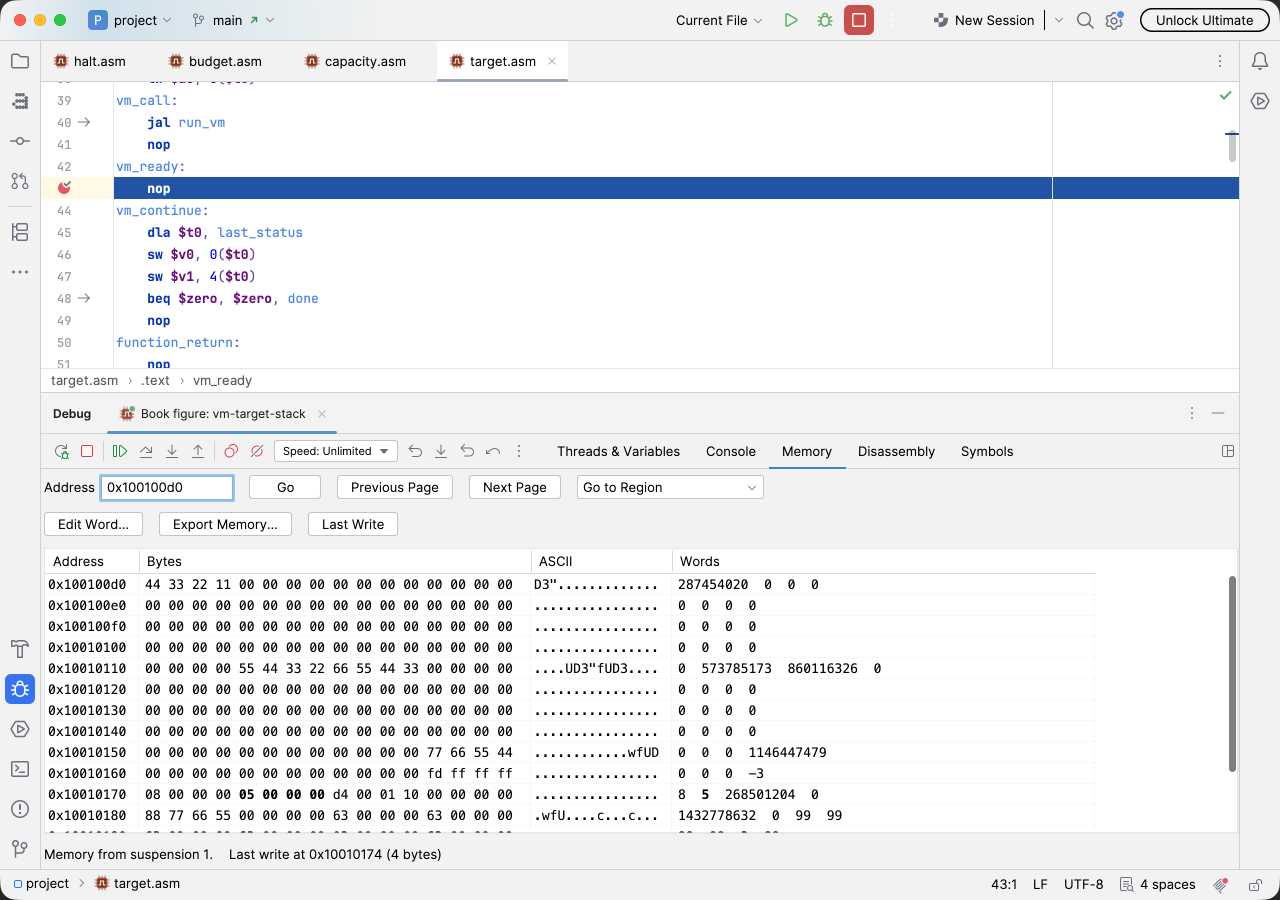
\includegraphics[artifact]{packages/018-tiny-bytecode-interpreter/captures/f04/stack.png}}
\sbox8{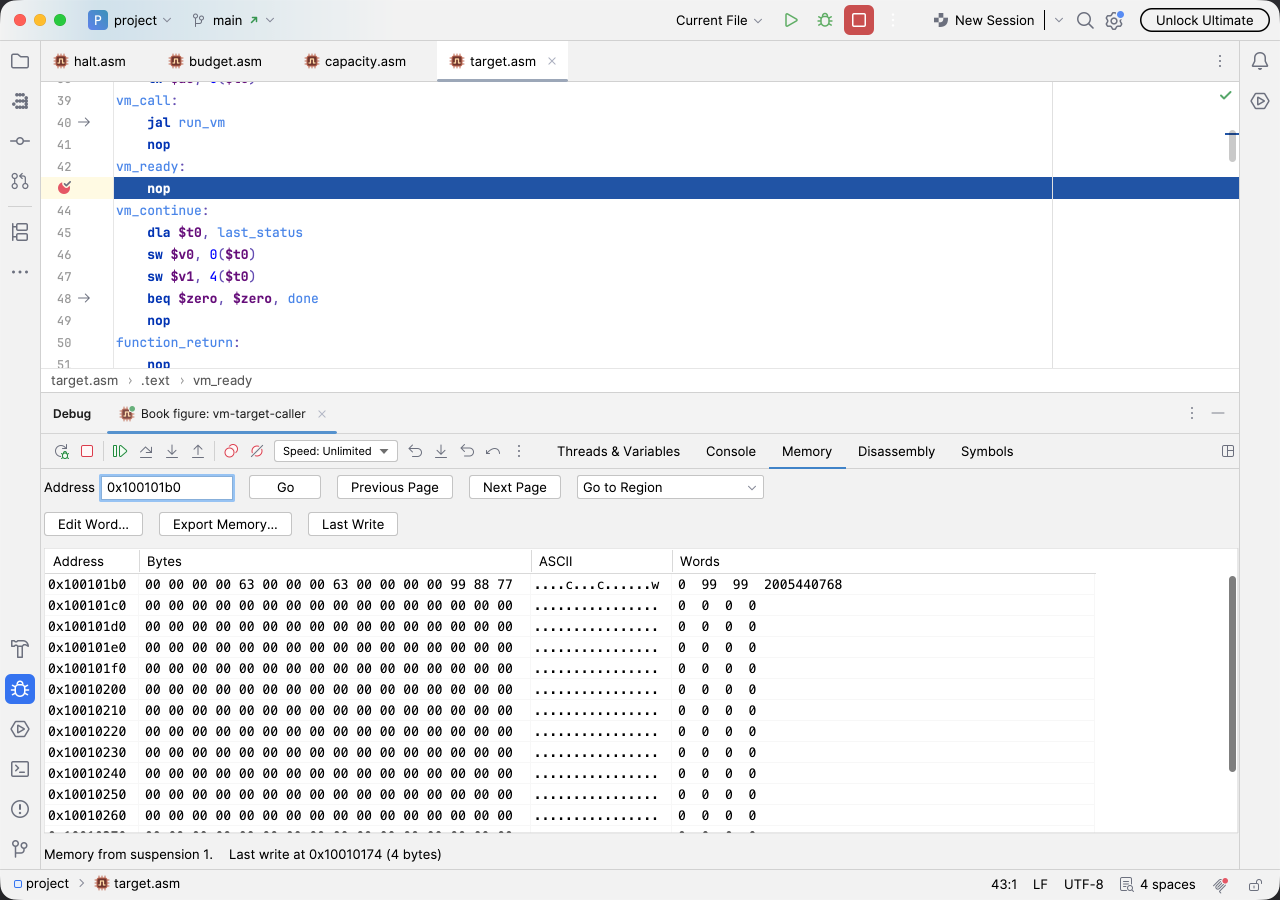
\includegraphics[artifact]{packages/018-tiny-bytecode-interpreter/captures/f04/caller.png}}
\edef\MARSvmtargetsourceLeft{\the\dimexpr0.036718750\wd0\relax}
\edef\MARSvmtargetsourceBottom{\the\dimexpr0.774444444\ht0\relax}
\edef\MARSvmtargetsourceRight{\the\dimexpr0.713281250\wd0\relax}
\edef\MARSvmtargetsourceTop{\the\dimexpr0.170000000\ht0\relax}
\edef\MARSvmtargetregistersLeft{\the\dimexpr0.246093750\wd0\relax}
\edef\MARSvmtargetregistersBottom{\the\dimexpr0.312222222\ht0\relax}
\edef\MARSvmtargetregistersRight{\the\dimexpr0.553906250\wd0\relax}
\edef\MARSvmtargetregistersTop{\the\dimexpr0.640000000\ht0\relax}
\edef\MARSvmtargetimageLeft{\the\dimexpr0.034375000\wd2\relax}
\edef\MARSvmtargetimageBottom{\the\dimexpr0.311111111\ht2\relax}
\edef\MARSvmtargetimageRight{\the\dimexpr0.584375000\wd2\relax}
\edef\MARSvmtargetimageTop{\the\dimexpr0.608888889\ht2\relax}
\edef\MARSvmtargetstateLeft{\the\dimexpr0.034375000\wd4\relax}
\edef\MARSvmtargetstateBottom{\the\dimexpr0.311111111\ht4\relax}
\edef\MARSvmtargetstateRight{\the\dimexpr0.584375000\wd4\relax}
\edef\MARSvmtargetstateTop{\the\dimexpr0.608888889\ht4\relax}
\edef\MARSvmtargetstackLeft{\the\dimexpr0.034375000\wd6\relax}
\edef\MARSvmtargetstackBottom{\the\dimexpr0.334444444\ht6\relax}
\edef\MARSvmtargetstackRight{\the\dimexpr0.584375000\wd6\relax}
\edef\MARSvmtargetstackTop{\the\dimexpr0.608888889\ht6\relax}
\edef\MARSvmtargetcallerLeft{\the\dimexpr0.034375000\wd8\relax}
\edef\MARSvmtargetcallerBottom{\the\dimexpr0.334444444\ht8\relax}
\edef\MARSvmtargetcallerRight{\the\dimexpr0.584375000\wd8\relax}
\edef\MARSvmtargetcallerTop{\the\dimexpr0.608888889\ht8\relax}
\begin{tikzpicture}[alt={Six annotated panels show branch-target validation failure before execution. Status minus three and retired count zero agree with descriptor PC zero, depth zero, retired zero, status minus three, capacity eight and fault five. The target operand at byte six is six and points into its own record. No operand is live; fuel is zero and caller result words remain 99.}]
\node[anchor=north west,inner sep=0,font=\small\bfseries] (source-title) at (6mm,0) {Next instruction after return};
\node[anchor=north west,inner sep=0] (source) at ([yshift=-1mm]source-title.south west) {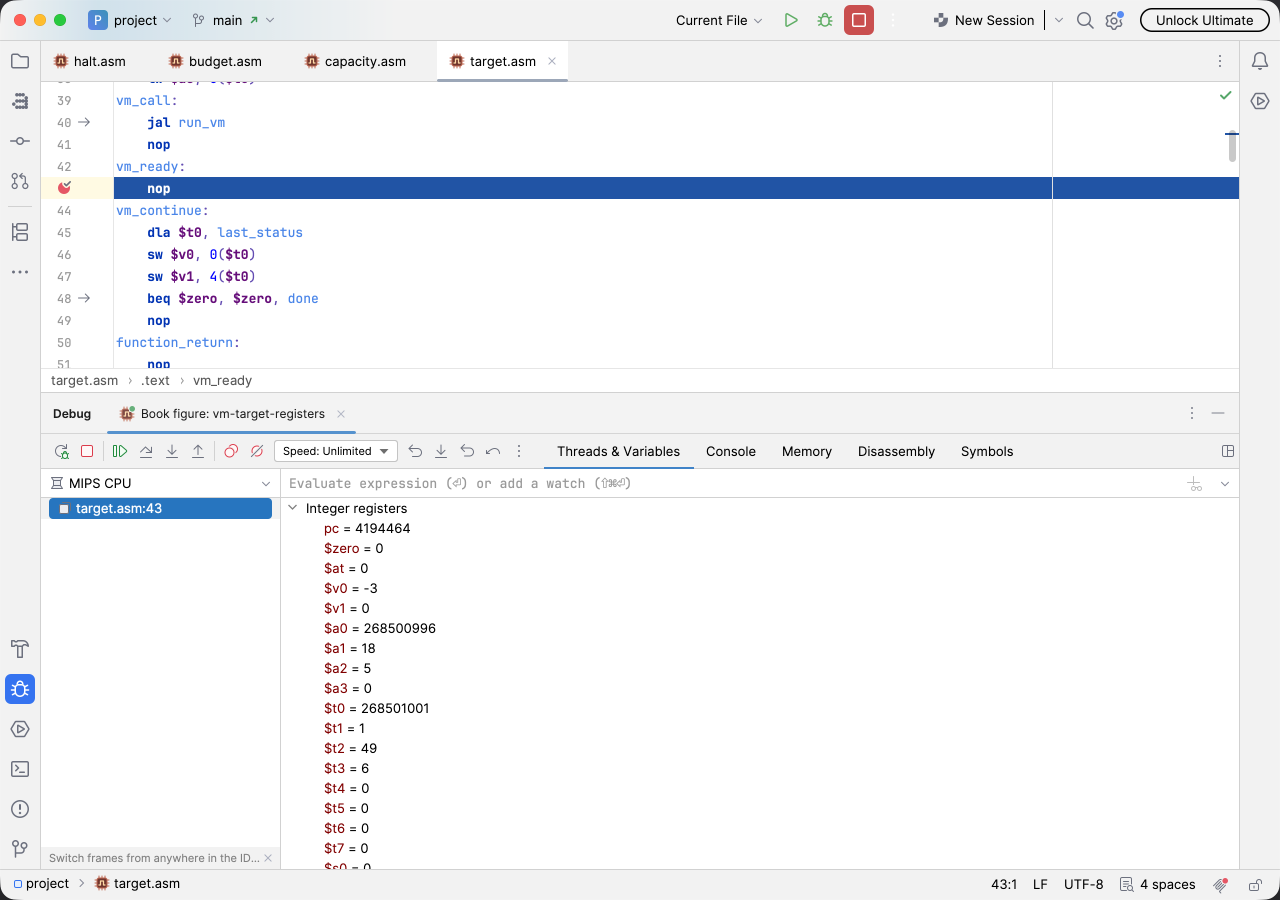
\includegraphics[width=0.54\linewidth,artifact,trim={\MARSvmtargetsourceLeft{} \MARSvmtargetsourceBottom{} \MARSvmtargetsourceRight{} \MARSvmtargetsourceTop{}},clip]{packages/018-tiny-bytecode-interpreter/captures/f04/registers.png}};
\begin{scope}[shift={(source.south west)},x={($(source.south east)-(source.south west)$)},y={($(source.north west)-(source.south west)$)}]
\draw[black,line width=0.7pt] (0.215625000,0.080000000) rectangle (0.384375000,0.520000000);
\node[draw=black,fill=white,circle,inner sep=1.5pt,font=\footnotesize] at ($(0.215625000,0.520000000)+(-3mm,0)$) {1};
\end{scope}
\node[anchor=north west,inner sep=0,font=\small\bfseries] (registers-title) at (0.58\linewidth,0 |- source-title.north) {Status and retired guest count};
\node[anchor=north west,inner sep=0] (registers) at ([yshift=-1mm]registers-title.south west) {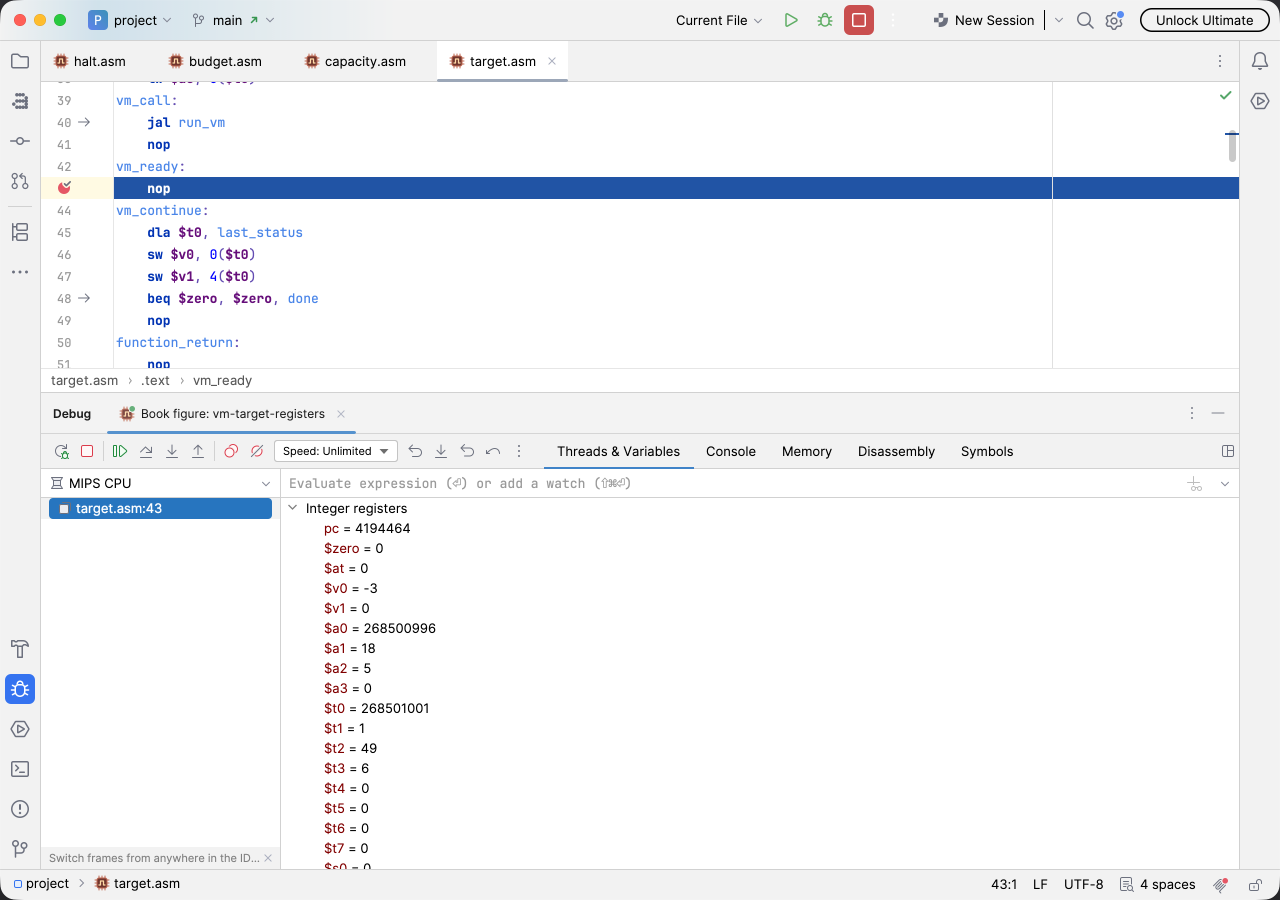
\includegraphics[width=0.42\linewidth,artifact,trim={\MARSvmtargetregistersLeft{} \MARSvmtargetregistersBottom{} \MARSvmtargetregistersRight{} \MARSvmtargetregistersTop{}},clip]{packages/018-tiny-bytecode-interpreter/captures/f04/registers.png}};
\begin{scope}[shift={(registers.south west)},x={($(registers.south east)-(registers.south west)$)},y={($(registers.north west)-(registers.south west)$)}]
\draw[black,line width=0.7pt] (0.023437500,0.023255814) rectangle (0.250000000,0.953488372);
\node[draw=black,fill=white,circle,inner sep=1.5pt,font=\footnotesize] at ($(0.023437500,0.953488372)+(-3mm,0)$) {2};
\end{scope}
\node[anchor=north west,inner sep=0,font=\small\bfseries] (image-title) at ([yshift=-1mm]source.south west) {Bytecode slice and surrounding bytes};
\node[anchor=north west,inner sep=0] (image) at ([yshift=-1mm]image-title.south west) {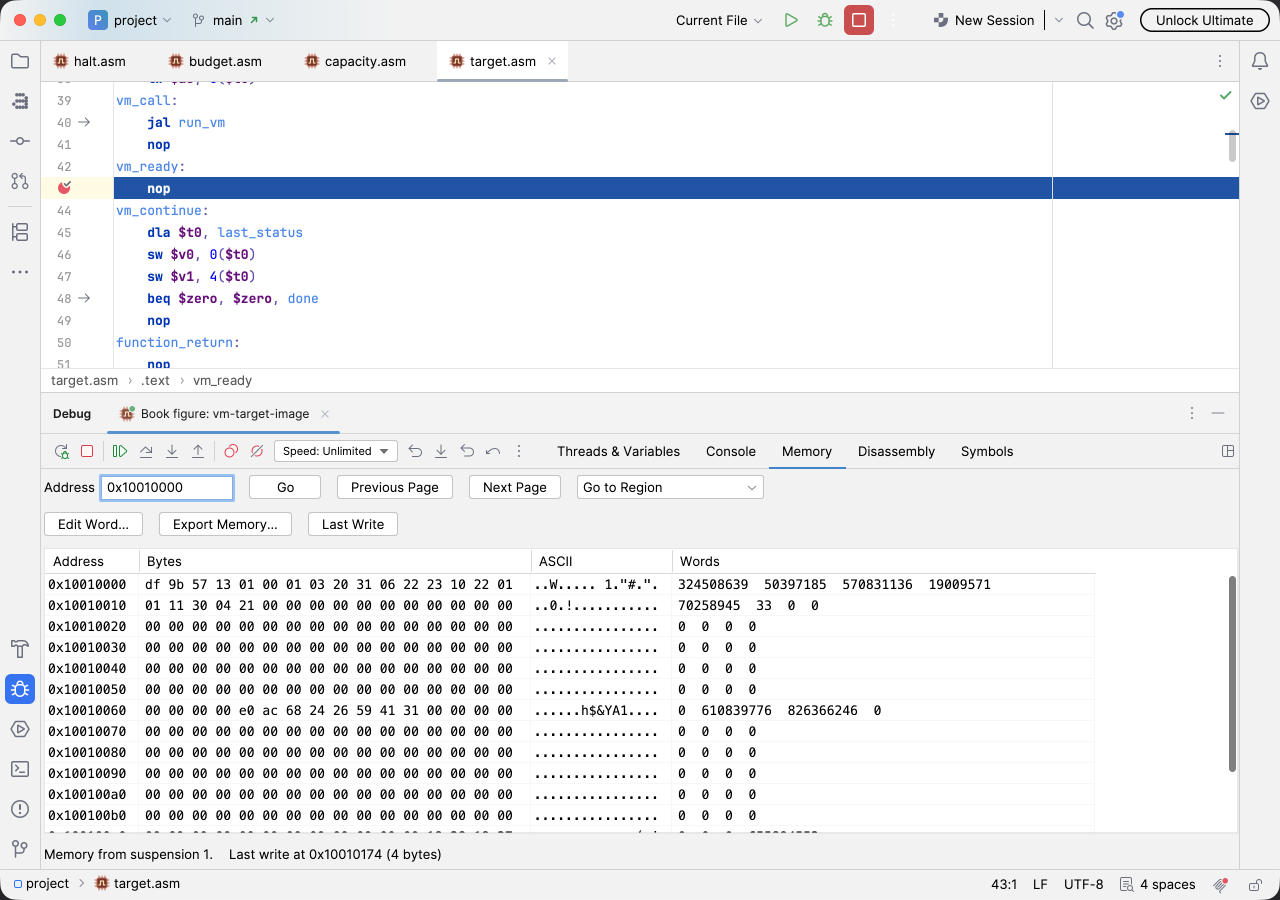
\includegraphics[width=0.84\linewidth,artifact,trim={\MARSvmtargetimageLeft{} \MARSvmtargetimageBottom{} \MARSvmtargetimageRight{} \MARSvmtargetimageTop{}},clip]{packages/018-tiny-bytecode-interpreter/captures/f04/image.png}};
\begin{scope}[shift={(image.south west)},x={($(image.south east)-(image.south west)$)},y={($(image.north west)-(image.south west)$)}]
\draw[black,line width=0.7pt] (0.194672131,0.055555556) rectangle (0.997950820,0.638888889);
\node[draw=black,fill=white,circle,inner sep=1.5pt,font=\footnotesize] at ($(0,0.638888889)+(-3mm,0)$) {3};
\end{scope}
\node[anchor=north west,inner sep=0,font=\small\bfseries] (state-title) at ([yshift=-1mm]image.south west) {Returned descriptor and preserved inputs};
\node[anchor=north west,inner sep=0] (state) at ([yshift=-1mm]state-title.south west) {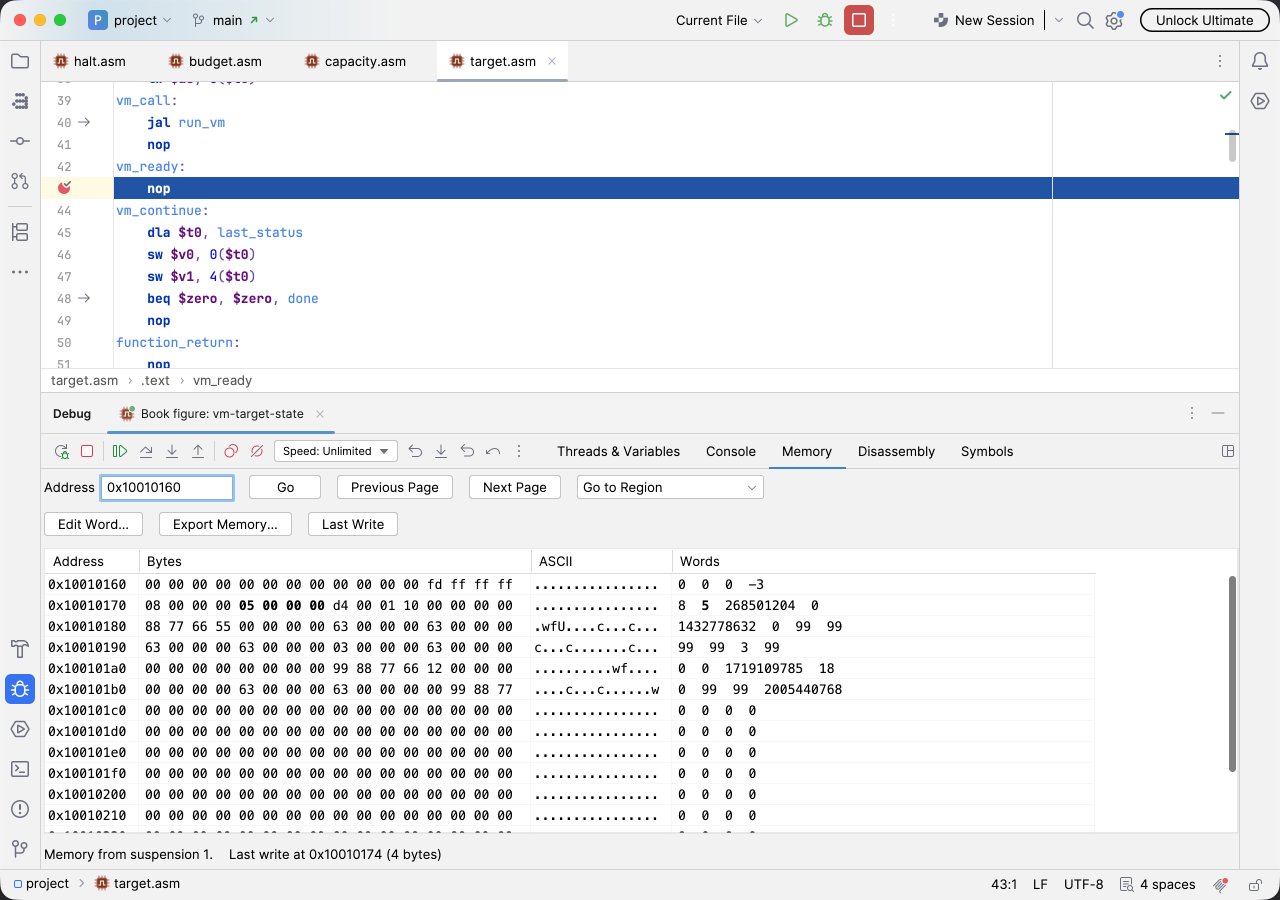
\includegraphics[width=0.84\linewidth,artifact,trim={\MARSvmtargetstateLeft{} \MARSvmtargetstateBottom{} \MARSvmtargetstateRight{} \MARSvmtargetstateTop{}},clip]{packages/018-tiny-bytecode-interpreter/captures/f04/state.png}};
\begin{scope}[shift={(state.south west)},x={($(state.south east)-(state.south west)$)},y={($(state.north west)-(state.south west)$)}]
\draw[black,line width=0.7pt] (0.194672131,0.055555556) rectangle (0.997950820,0.638888889);
\node[draw=black,fill=white,circle,inner sep=1.5pt,font=\footnotesize] at ($(0,0.638888889)+(-3mm,0)$) {4};
\end{scope}
\node[anchor=north west,inner sep=0,font=\small\bfseries] (stack-title) at ([yshift=-1mm]state.south west) {Physical operand cells after return};
\node[anchor=north west,inner sep=0] (stack) at ([yshift=-1mm]stack-title.south west) {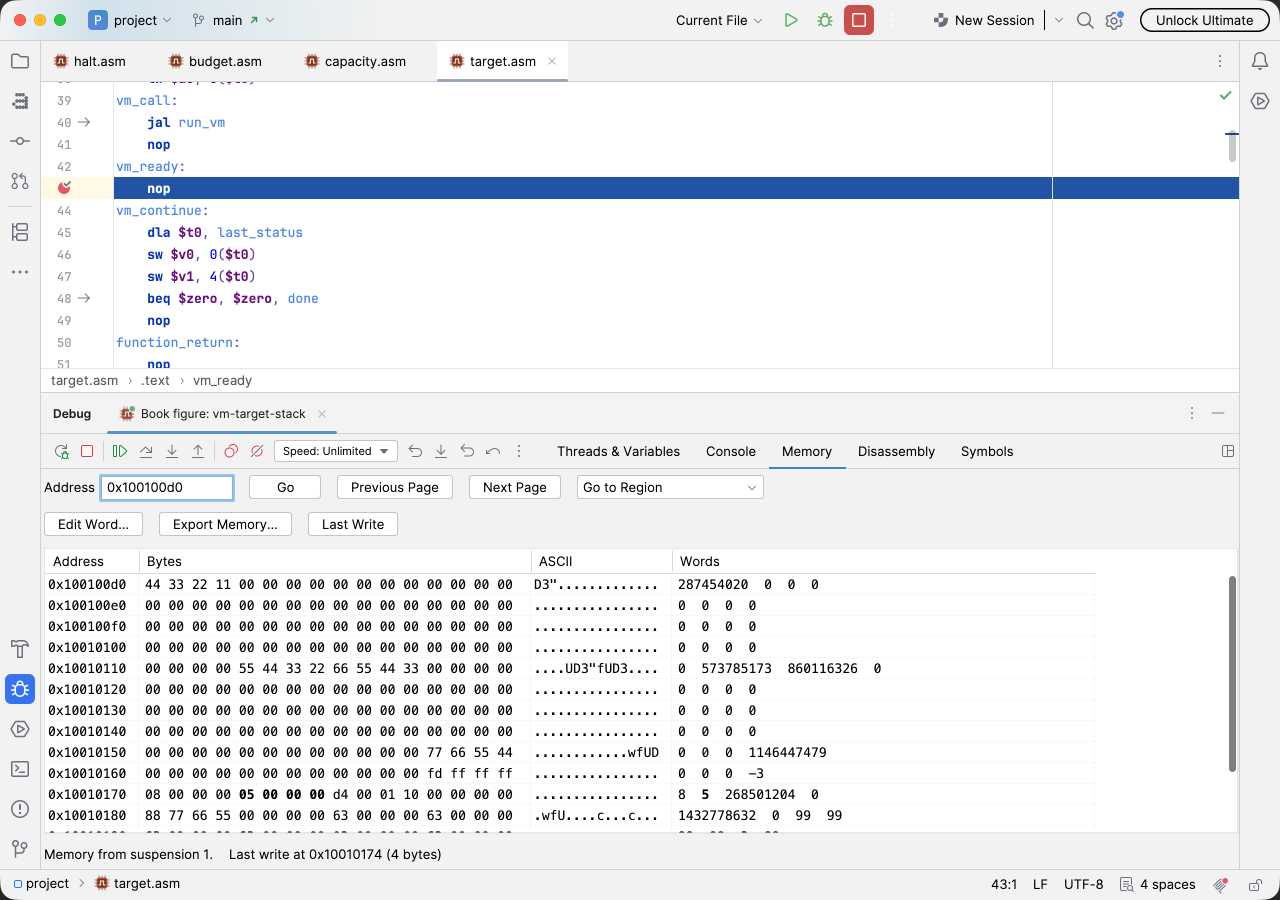
\includegraphics[width=0.84\linewidth,artifact,trim={\MARSvmtargetstackLeft{} \MARSvmtargetstackBottom{} \MARSvmtargetstackRight{} \MARSvmtargetstackTop{}},clip]{packages/018-tiny-bytecode-interpreter/captures/f04/stack.png}};
\begin{scope}[shift={(stack.south west)},x={($(stack.south east)-(stack.south west)$)},y={($(stack.north west)-(stack.south west)$)}]
\draw[black,line width=0.7pt] (0.194672131,0.078431373) rectangle (0.997950820,0.490196078);
\node[draw=black,fill=white,circle,inner sep=1.5pt,font=\footnotesize] at ($(0,0.490196078)+(-3mm,0)$) {5};
\end{scope}
\node[anchor=north west,inner sep=0,font=\small\bfseries] (caller-title) at ([yshift=-1mm]stack.south west) {Budget and caller result words};
\node[anchor=north west,inner sep=0] (caller) at ([yshift=-1mm]caller-title.south west) {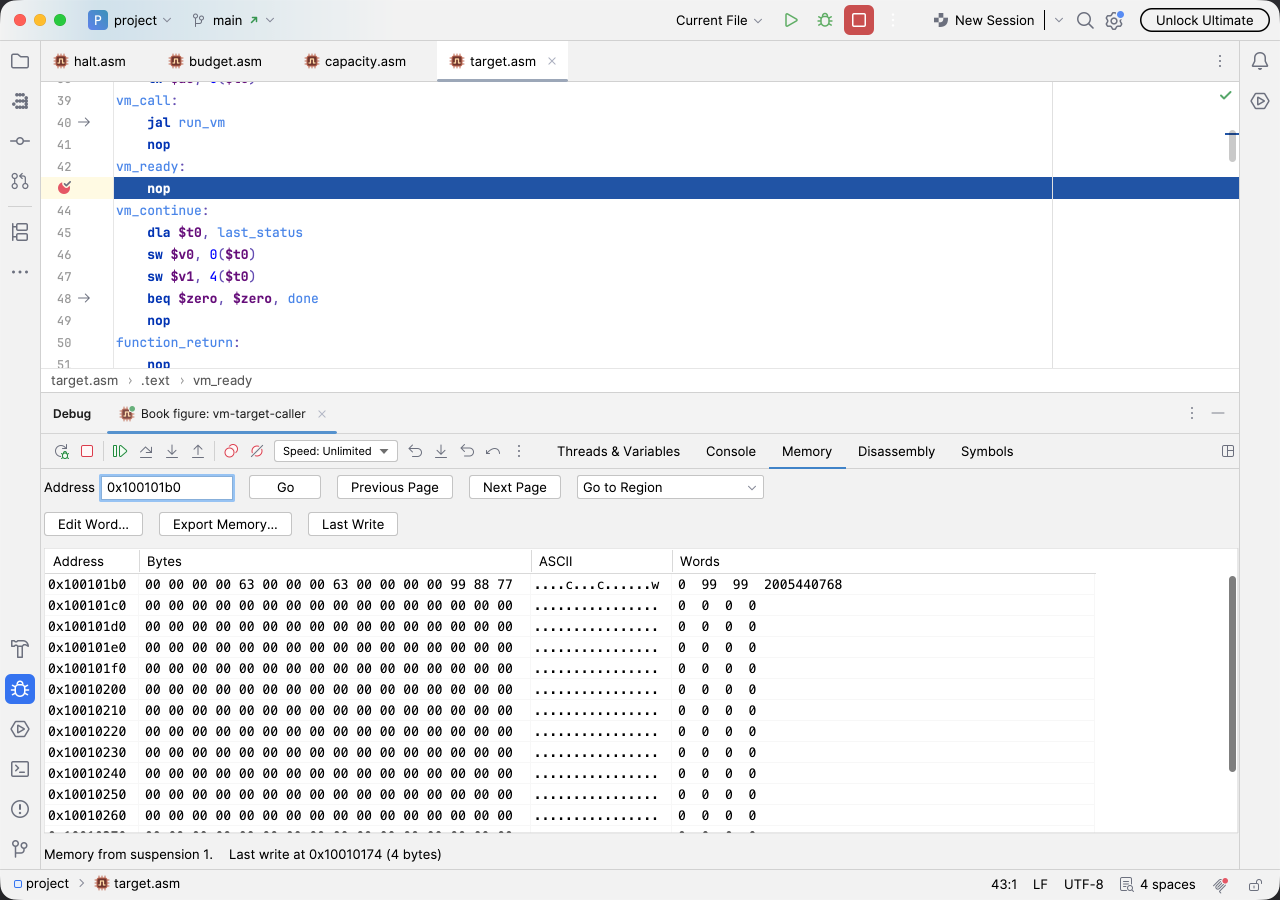
\includegraphics[width=0.84\linewidth,artifact,trim={\MARSvmtargetcallerLeft{} \MARSvmtargetcallerBottom{} \MARSvmtargetcallerRight{} \MARSvmtargetcallerTop{}},clip]{packages/018-tiny-bytecode-interpreter/captures/f04/caller.png}};
\begin{scope}[shift={(caller.south west)},x={($(caller.south east)-(caller.south west)$)},y={($(caller.north west)-(caller.south west)$)}]
\draw[black,line width=0.7pt] (0.194672131,0.078431373) rectangle (0.997950820,0.490196078);
\node[draw=black,fill=white,circle,inner sep=1.5pt,font=\footnotesize] at ($(0,0.490196078)+(-3mm,0)$) {6};
\end{scope}
\end{tikzpicture}
\par\smallskip
\begin{minipage}{\linewidth}
\small
\begin{enumerate}
\setlength{\itemsep}{2pt}
\setlength{\parsep}{0pt}
\item The blue \texttt{nop} at \texttt{vm\_ready} follows the function return. Descriptor outputs are published; the caller\textquotesingle s separate result stores are still ahead.
\item \texttt{\$v0 = -3} reports invalid branch target; \texttt{\$v1 = 0} confirms no guest instruction retired. A zero budget still requires complete structure and target validation. Budget exhaustion applies only after those phases succeed.
\item The changed bytes \texttt{31 06} begin at decimal offset five. The target value 6 names the operand byte at offset six, not an instruction beginning. Target validation rejects it even though execution has not tested a stack value.
\item The descriptor contains PC 0, depth 0, retired 0 and status $-3$. Fault 5 identifies the invalid branch record. The two offsets differ because execution never began: fault names the validation problem while PC retains the initial execution position.
\item Every displayed operand cell is zero, but depth 0 means none is live. The interpreter makes no operand-stack stores on this validation failure. Capacity 8 and the stack pointer remain inputs; they do not imply that eight zero operands exist.
\item Fuel precedes the caller\textquotesingle s two result words and guard. Both results still contain 99 (\texttt{63 00 00 00}); continuing copies \texttt{v0} and \texttt{v1} into them.
\end{enumerate}
\end{minipage}
\caption{An invalid encoded target is rejected before a zero instruction budget.}
\label{capture:018-tiny-bytecode-interpreter-f04}
\label{vm-f04}
\end{figure}
\par
